% !TEX root = 0_main.tex
\chapter{Compacting Privacy-Preserving k-Nearest Neighbor Search using Logic Synthesis}\label{chap:knn}
In this appendix, we discuss solving privacy-preserving $k$-nearest neighbor ($k$-NN) search using Yao's \acrshort{gc} protocol.
We use the \gls{tinygarble} \acrshort{gc} synthesis method to implement $k$-NN in optimized and compact circuits for \acrshort{gc}.

In this appendix, we first introduce the problem of privacy-preserving $k$-NN and the challenge of solving it using Yao's \acrshort{gc} protocol.
Next, we provide the related work in the literature about privacy-preserving $k$-NN and methods for generating optimized and compact circuits for $k$-NN.
We then explain our approach that is based on \gls{tinygarble} sequential circuit synthesis (see \chap{chap:seq}).
Lastly, we provide the evaluation results and conclude the appendix.
A version of this appendix has been published in 2015 Proceedings of the 52nd Annual Design Automation Conference (DAC) \cite{songhori2015compacting}.

\section{Introduction and Motivation}\label{sec:knn-intro}
%What is the problem?
%KNN-search
The search for similarities has a wide range of applications in data mining, such as finding close matches in images, local features, biological and genome data, and multimedia systems \cite{qi2008efficient}.
The most extensively used function for similarity search is the $k$-nearest neighbor ($k$-NN).
For a given dataset $S$ of $n$ points in a multi-dimensional space $w$, and a query $q$, the $k$-NN search finds a subset of $S$ with $k$ points that are closest to $q$.
Numerous works have focused on development of efficient $k$-NN search, where the underlying assumption is that the dataset $S$ and the query point $q$ are public.
For example, it is well known that the approximate search speed of $k$-NN can be dramatically improved by projecting the data into smaller hash tables \cite{andoni2006near,weiss2009spectral}.
However, such approximation methods are orthogonal to our effort.
We focus on the basic textbook $k$-NN search which could also be accelerated with the known approximations.

%private NN-search
In a number of scenarios, the data and the query are sensitive and it is important to maintain privacy while performing the search.
This has motivated the development of privacy-preserving $k$-NN search \cite{shaneck2009privacy}.
The existing works assume that the parties each own a private dataset, while the query $q$ is not private; they focus on devising higher-level protocols for privacy-preserving similarity search and proofs of privacy \cite{shaneck2009privacy,qi2008efficient}.
These works mostly leverage Homomorphic encryption to perform a \acrfull{sfe}.
Homomorphic encryption enciphers the data (\emph{plaintext}) in such a way that performing a mathematical function on the encrypted information, and then decrypting the result, produces the same answer as performing an analogous operation on the plaintext.
Since the first fully homomorphic encryption was proposed about 5 years ago \cite{gentry2009fully}, numerous protocol-level and implementation-level advancements have been made.
Even so, the implementations are still rather inefficient and impracticable for real applications.

%Yao's GC
In this appendix, we suggest the first efficient and scalable methodology for privacy-preserving $k$-NN search that is implementable on embedded processors.
In contrast to the existing literature that assumes private datasets and known query, we assume a more general case of both private dataset and private query.
Our methodology for providing a \acrshort{sfe} is based on Yao's \acrfull{gc} that is currently considered the most effective way to preserve privacy \cite{huang2012private,brenner2011hcrypt}.
Note that the use of \acrshort{gc} for the generic problem of privacy preserving data mining has been proposed, but not implemented \cite{agrawal2000privacy}.
The \acrshort{gc} protocol requires that the function is represented as a binary circuit.
It encrypts the truth tables of Boolean gates in the circuit.
The input values are used as to decrypt the output value of the gates.
All the garbled circuits suggested to date only support one pass, directed acyclic circuits, \emph{a.k.a., combinational circuits}.
The only available implementation of the privacy-preserving similarity search using the \acrshort{gc} protocol is for the 1-NN search, where the circuit size was linearly increasing with the dataset size \cite{kolesnikov2009improved}.
This increase is due to the fact that conventional combinational logic representation is not scalable.

%what has been done
To implement a \acrshort{gc}, one needs to compile the higher-level description of the functions to the Boolean logic suitable for garbling.
For this purpose, several custom compilers have been developed by the security and software/compiler communities \cite{malkhi2004fairplay,henecka2010tasty,holzer2012secure,kreuter2013pcf}.
These compilers either use a custom library for a general purpose programming language \cite{malkhi2004fairplay}, or introduce transformations for performing compile-time circuit garbling and on-the-fly gate generation \cite{kreuter2013pcf}.
Since these compilation methods are built upon the combinational logic model, they all suffer from the scalability issue.

%Sequential methodology and logic synthesis
Our work is the first to synthesize and optimize the \acrshort{gc} for performing privacy preserving $k$-NN using a sequential representation.
Instead of relying on custom compilers, we follow \gls{tinygarble} synthesis methodology proposed in \chap{chap:syn} and \chap{chap:seq}.
In those chapters, we view the compilation of the general sequential circuit as a special case of logic synthesis.
By defining new custom libraries and design objective/constraints, we demonstrate that utilizing standard logic synthesizers addresses the challenges in privacy preserving $k$-NN.
As a result, we can store the \acrshort{gc} and perform the privacy preserving $k$-NN search with an unprecedented efficiency.

\textbf{Problem Statement.} Alice has a query $q$ and Bob has a dataset $S$.
They want to jointly compute the $k$ nearest neighbors of $q$ in $S$ such that Bob does not learn anything about $q$ and Alice does not learn anything about $S$ except the nearest neighbors.

\textbf{Contributions.} In brief, our contributions are as follows:

%Contribution
\begin{itemize}
  \item Introducing the first efficient, practicable, and scalable methodology for privacy-preserving $k$-NN search assuming that the dataset and query are each privately held.
  The method is based on the Yao's \acrshort{gc} protocol and implementable on embedded processors.

  \item Proposing a sequential circuit description for privacy-preserving $k$-NN search using Yao's Garbled Circuit protocol (instead of the known combinational representation).
  New transformations are created such that the sequential $k$-NN implementation are securely evaluated by interfacing with the available (combinational) cryptographic garbling schemes.

  \item Development of new custom libraries to generate optimized circuits for $k$-NN search using the standard logic synthesis tools.
  This is the first time that conventional logic synthesis is utilized for secure function evaluation of $k$-NN.

  \item Reduction in the size of the required memory for \acrshort{gc} from $\BigO{nw}$ to $\BigO{w}$ compared with the best known \acrshort{gc} implementation of 1-NN \cite{kolesnikov2009improved}.
  Our scalable implementation requires a memory in the order of $\BigO{kw}$ for $k$-NN search.
  Note that $k$-NN search was impracticable earlier (for large $n$) due to the linear growth of the combinational representation.

  \item Proof-of-concept implementation of privacy preserving $k$-NN utilizing the Synopsys Design Compiler on an Intel processor.
  For example, the circuit size for $k$-NN search with $w=31, k=8$ is only 41.8KB.
\end{itemize}

\section{Related Work}\label{sec:knn-related}
The related literature in realizing privacy-preserving $k$-NN search has mainly focused on using homomorphic encryption as the enabling cryptographic primitive \cite{shaneck2009privacy,qi2008efficient}.
In their protocol, two parties perform $k$-NN search locally on their respective private dataset for a public query and then privately combine their results to form the $k$-NN.
In contrast with these works, we adopt a more general setting in which one party holds a private dataset and the other one provides a private query.
Moreover, we only rely on Yao's \acrshort{gc} protocol which is known to be much more efficient \acrshort{sfe} protocol than homomorphic encryption \cite{huang2012private,brenner2011hcrypt}.
The use of \acrshort{gc} for privacy preserving data mining has been suggested, but the existing literature focused on theoretical/protocol aspects and not implementation \cite{agrawal2000privacy}.
Leveraging our sequential description, this paper proposes the first scalable implementation and a low-overhead realization of secure $k$-NN on a conventional processor.

The work on generating Boolean functions for \acrshort{gc} can be broadly classified into three categories: cryptographic primitives such as \cite{malkhi2004fairplay,bellare2013efficient}, transformations at the logic-level such as \cite{kolesnikov2008improved}, and compiler/software techniques for mapping \acrshort{gc} to the Boolean logic including \cite{malkhi2004fairplay,holzer2012secure,kreuter2013pcf}.
Our work is orthogonal to the advances in the \acrshort{gc} cryptographic primitives and logic-level transformations.
We provide a compilation from the functional description to the Boolean logic which can be optimized and interfaced for any \acrshort{gc} scheme.
Therefore, we only describe the related work in the area of compiler/software techniques.

In the area of mapping and optimizing functions into Boolean logic for \acrshort{gc}, the related literature has suggested developing custom compilers \cite{malkhi2004fairplay,henecka2010tasty,holzer2012secure,kreuter2013pcf}, custom libraries for conventional high-level compilers \cite{huang2011faster,malka2011vmcrypt,henecka2013faster}, hardware accelerators\cite{pu2013computing,jarvinen2010garbled,bellare2013efficient}, and mobile device implementation \cite{mood2012memory}.

Following the introduction of the first compiler for \acrshort{gc}, called Fairplay \cite{malkhi2004fairplay}, a number of researchers have focused on providing a custom compiler to interpret high level procedural language and map it to a circuit description language \cite{henecka2010tasty,holzer2012secure}.
The most scalable existing compiler is \gls{pcf}, which introduces loops that, if given manually in the high level language, are kept until the \acrshort{gc} evaluation \cite{kreuter2013pcf}.
Our sequential description of the $k$-NN function that we input in the \acrshort{hdl} format is much more compact than the high-level (software) loop embracing in \gls{pcf}.
Note that \gls{pcf} is also based upon a combinational description.

Another class of proposed \acrshort{gc} compilation methods leverage a library-based technique along with conventional software compilers.
Some examples include FastGC \cite{huang2011faster}, VMCRYPT \cite{malka2011vmcrypt}, and FastGC extension to re-usable sub-circuits \cite{henecka2013faster}.
We are the first to adapt a hardware description language and conventional logic synthesis for the important problem of privacy preserving of $k$-NN.
Our method is automated, while it also benefits from custom logic-level libraries.

A number of researchers have suggested development of hardware accelerators for \acrshort{gc}, including \acrshort{gpu}s \cite{husted2013gpu,pu2013computing}, \acrshort{fpga}s \cite{jarvinen2010garbled}, or using the \acrshort{aes-ni} available in recent CPUs \cite{bellare2013efficient}.
Our work is orthogonal to this domain and can benefit from building accelerators for our sequential representation.

Using the \acrshort{gc} for secure computing on resource constrained devices such as mobile/embedded platforms was suggested in \cite{huang2011privacy}.
A recent work in this area described a protocol for \acrshort{gc} that relies on a smartcard embedded in the mobile device \cite{demmler2014ad}.
These implementations can greatly benefit from the scalable and efficient $k$-NN methodology introduced in this thesis.
To overcome the limitations of resource-constrained devices, a set of relevant work in this area suggested outsourcing the \acrshort{gc} generation and evaluation to cloud servers \cite{carter2016secure,carter2014whitewash}.
Our work demonstrates the feasibility of on-device \acrshort{gc} implementation.

\section{Nearest Neighbors Search Circuit}\label{sec:knn-circuit}
In this section, we present implementation of privacy-preserving $k$-NN search using Yao's \acrshort{gc} protocol.
First, we describe the optimized circuit generation for \acrshort{gc} using logic synthesis tools.
Next, we outline the implementation of 1-NN search using conventional \acrshort{gc} based on combinational circuit.
Lastly, we discuss the compact realizations of 1-NN and $k$-NN search based on sequential circuit.

Without any loss of generality, we assume the distance function for finding the nearest neighbors is Hamming distance in the following description.

\subsection{Circuit Generation}\label{ssec:knn-circuitgen}
We customize the flow of the standard logic synthesis tools to generate circuits optimized for \acrshort{gc} protocol.
As mentioned in \chap{chap:prelim} for \acrshort{gc} with Free XOR optimization, there is a need to minimize the number of non-XOR gates in the Boolean representation.
We perform two major customization in the synthesis flow.
First, we create a new \emph{synthesis library} to aid the conversion of the arithmetic and conditional operations to \acrshort{gc}-optimized logical modules.
Second, we develop a \emph{technology library} to guide the mapping of the logic to the circuit netlist.

\subsubsection{Synthesis Library}
To realize the $k$-NN search, a set of basic arithmetic and conditional operations consisting of comparator, multiplexer, and Hamming distance are required.
We create a custom synthesis library that includes the minimum non-XOR implementations of these operations.
A $w$-bit comparator ($\mathit{COMP}_w$) is implemented using only $w$ non-XOR gates \cite{kolesnikov2009improved}.
A $w$-bit multiplexer ($\mathit{\acrshort{mux}}_w$) is realized using $w$ non-XOR gates \cite{kolesnikov2008improved}.
A $w$-bit Hamming distance ($\mathit{HAMMING}_w$) is devised using $w-\lceil \log _2(w) \rceil$ non-XOR gates where $w=2^k-1, k \in \mathbb{N}$ \cite{boyar2006concrete}.
In all these modules, the total number of gates is $\BigO{w}$.

\subsubsection{Technology Library}
The technology library includes logical descriptions of basic units and their parameters like delay and area.
The synthesis tool uses the technology library to generate a circuit optimized for given objectives and constraints.
We design a custom technology library that contains 2-input gates (according to the requirement of the \acrshort{gc} protocol).
We set the area of XOR gates to 0 and the area of non-XOR gates to 1.
The circuits are synthesized with the area constraint set to 0 so that the synthesis tool's objective becomes minimizing the number of non-XOR gates in the generated circuit.

An additional feature of this library is inclusion of non-standard gates (other than basic gates like NOT, AND, NAND, OR, NOR, XOR, and XNOR) to increase the flexibility of the mapping process.
For example, the logical functions $F = A\vee B$ and $F = (\sim A)\vee B$ requires equal time in garbling/evaluation.
However, using only standard gates the second function will require a NOT gate and an OR gate.
We include four such non-standard gates which have an inverted input.

\subsection{Combinational Garbled Circuit}\label{ssec:knn-combgc}
As stated in \chap{chap:prelim}, all previous implementations of \acrshort{gc} protocol use a combinational description.
To start our implementation for the special case of 1-NN search, we look for the closest point ($o$) to the query point ($q$) in the dataset ($S$).
In the privacy-preserving setting, there is a need to compare the query point to all the points in the dataset.
This is because the (private) intermediate search values cannot be utilized to bound the search, e.g., binary search.

\fig{fig:fist-nns-comb} shows the combinational circuit for $1$-NN.
The implementation uses $n$ Hamming distance modules, and $n-1$ \emph{min} modules (consisting of 1 COMP and 2 \acrshort{mux}s) to find the nearest point.
One \acrshort{mux} selects the smaller distance for later comparison while the other one finds the point corresponding to that distance.

\begin{figure}
\centering
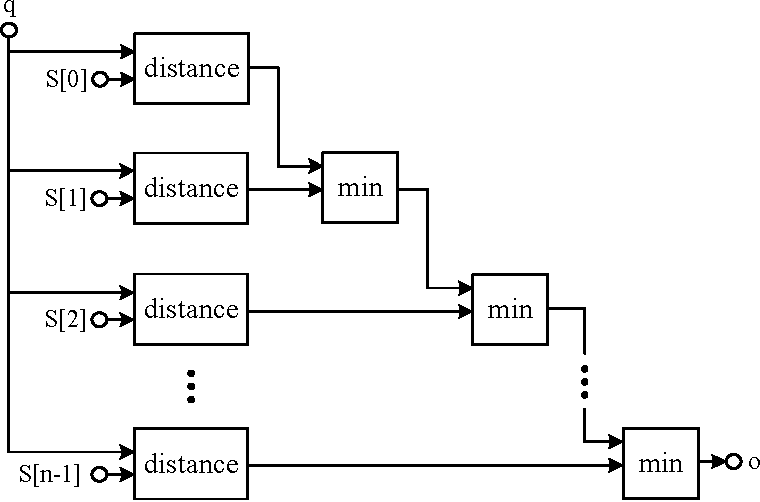
\includegraphics[width=0.8\textwidth]{first-nns-comb-crop.pdf}
\caption{Combinational circuit for $1$-NN.
It consists of $n$ Hamming distance and $n-1$ min modules.}
\label{fig:fist-nns-comb}
\end{figure}

The total number of gates in the 1-NN combinational circuit is as follows:
\begin{align*}
\text{\# of gates} =& ~	n \times \mathit{HAMMING}_{w}\\
					& + (n-1) \times (\mathit{COMP}_{\lceil \log _2(w) \rceil} \\
					& + \mathit{\acrshort{mux}}_w + \mathit{\acrshort{mux}}_{\lceil \log _2(w)} \rceil)\\
\Rightarrow \text{\# of gates} \in & ~\BigO{nw}.
\end{align*}

The circuit should be garbled/evaluated only once.
Thus, the time complexities of garbling/evaluation is $\BigO{nw}$.

\subsection{Sequential Garbled Circuit}\label{ssec:knn-seqgc}
Sequential circuits can be used as a very compact circuit description for both real hardware and \acrshort{gc} protocol.
A sequential circuit is composed of a combinational circuit and a set of registers that stores the intermediate values.
We modify the garbling scheme such that for each sequential cycle, it garbles/evaluates the combinational part and stores the garbling keys for the registers.
The stored keys are used as inputs in the next cycle.
To ensure security, each gate should have a unique identifier for each time that it is garbled/evaluated.
Since in the sequential circuit each gate is garbled/evaluated multiple times, we use the combination of gate index and cycle index as a unique identifier for each gate invocation.
Thereby, the proof of security provided in \cite{lindell2009proof,bellare2013efficient} also applies to our garbling scheme.
We now describe the sequential 1-NN search implementation followed by $k$-NN implementation.

\subsubsection{Sequential 1-NN}
Our 1-NN search sequential circuit is implemented with only 1 Hamming distance and 1 min module.
\fig{fig:fist-nns-seq} illustrates the sequential circuit for $1$-NN search.
In each cycle $c$, the circuit computes the distance between $q$ and $S[c]$.
Next, it compares the resulting distance with the stored minimum distance in the register (reg).
It then stores the minimum distance along with the nearest point until cycle $c$.
The total number of cycles required to compute 1-NN is $n$.

\begin{figure}
\centering
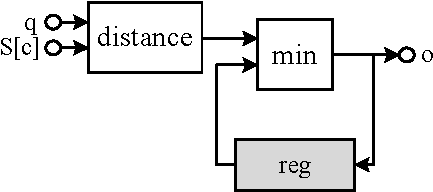
\includegraphics[width=0.5\textwidth]{first-nns-seq-crop.pdf}
\caption{Sequential circuit for $1$-NN.
It consists of 1 Hamming distance and 1 min module.
For a dataset of size $n$, the circuit is required to be garbled/evaluated $n$ times.}
\label{fig:fist-nns-seq}
\end{figure}

The total number of gates in the 1-NN sequential circuit is as follows:
\begin{align*}
\text{\# of gates}=	& ~ \mathit{HAMMING}_{w}\\
					& + (\mathit{COMP}_{\lceil \log _2(w) \rceil} \\
					& + \mathit{\acrshort{mux}}_w + \mathit{\acrshort{mux}}_{\lceil \log _2(w)} \rceil)\\
\Rightarrow \text{\# of gates} \in & ~ \BigO{w}.
\end{align*}

The circuit should be garbled/evaluated $n$ times.
Thus, the time complexities of garbling/evaluation are the same as the combinational circuit and equal to $\BigO{nw}$.

\subsubsection{Sequential k-NN}
In $k$-NN search, the goal is to find the $k$ nearest points to the query in the dataset.
We expand the sequential circuit for the 1-NN to store the $k$ nearest points.
For this purpose, we implement a priority queue with depth of $k$ which receives one point at each cycle.
The priority of each point is equal to its distance to the query.
\fig{fig:k-nns-seq} shows the sequential circuit for the $k$-NN search.
The circuit has 1 Hamming distance, $k$ min, and $k-1$ \emph{max} modules.
The max module, like min, consists of 1 COMP and 2 \acrshort{mux}s.

\begin{figure}
\centering
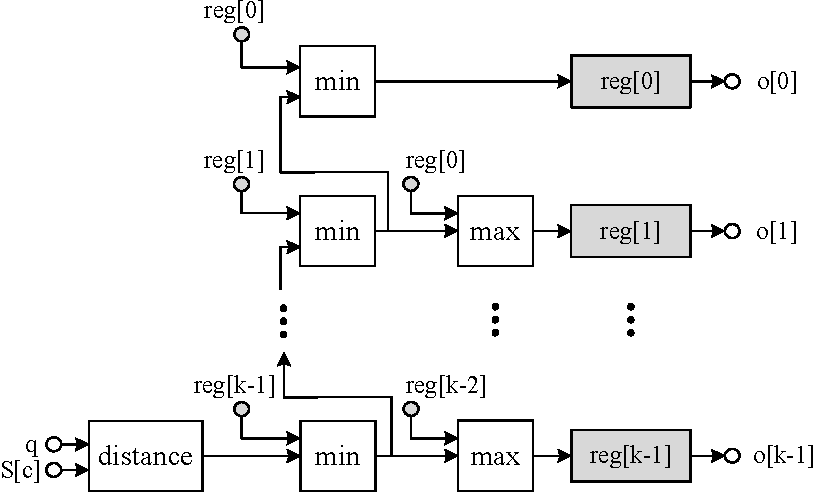
\includegraphics[width=0.8\textwidth]{k-nns-seq-crop.pdf}
\caption{Sequential circuit for $k$-NN.
It consists of 1 Hamming distance, $k$ min, and $k-1$ max modules.
It requires to be evaluated $n$ times where $n$ is the size of the dataset $S$.}
\label{fig:k-nns-seq}
\end{figure}

The total number of gates in the 1-NN sequential circuit is as follows:
\begin{align*}
\text{\# of nonXORs}=			& ~ \mathit{HAMMING}_{w}\\
								& + (2k-1) \times \mathit{COMP}_{\lceil \log _2(w) \rceil} \\
								& + (2k-1) \times (\mathit{\acrshort{mux}}_w  + \mathit{\acrshort{mux}}_{\lceil \log _2(w) \rceil})\\
\Rightarrow \text{\# of nonXORs} \in & ~ \BigO{kw}.
\end{align*}

The circuit should be garbled/evaluated $n$ times.
Thus, the time complexities of garbling/evaluation are the same as the combinational circuit and equal to $\BigO{nkw}$.
Note that due to the unscalability of combinational $k$-NN search, we did not include its implementation.

\section{Evaluation}\label{sec:knn-eval}
The circuit generation is done with Synopsis Design Compiler (DC) 2010.03-SP4.
We also use the Synopsis Library Compiler from DC package to interpret our custom technology libraries.
For garbling and evaluation we use the JustGarble framework \cite{bellare2013efficient} which we modified to support sequential circuits.
JustGarble exploits the cryptographic permutations realizable by fixed-key AES for \acrshort{gc} operations.
We run the framework on a system with Ubuntu 14.10 Desktop, 12GB of memory, and Intel Core i7-2600 CPU at 3.4GHz to assess the timing performance.

The metrics used to evaluate the performance of our implementations are as follows:
\begin{itemize}
  \item The Circuit Size ($\mathit{CS}$) in Bytes is computed as $$\mathit{CS} = 24\times q, $$ where $q$ is total number of gates.
We store 2 indices ($16$B) and one type ($8$B) for each gate in circuit description file.

  \item Circuit Size Efficiency ($\mathit{CSE}$) is defined as $$\mathit{CSE} = \dfrac{\mathit{CS}_{C}}{\mathit{CS}_{S}}, $$ where $\mathit{CS}_{C}$ is the size of the combinational circuit and $\mathit{CS}_{S}$ is that of the sequential circuit.

  \item The garbling time is calculated as $$\mathit{T} = \text{\# of non-XOR} \times \mathit{T_{nonXOR}} + \text{\# of XOR} \times \mathit{T_\text{XOR}},$$ where $\mathit{T_{nonXOR}}$ is the execution of a non-XOR gate and $\mathit{T_\text{XOR}}$ is the execution of a XOR gate, which are $164$ clock cycles (cc) and $62$cc respectively in the specified system.
We measured these values as the mean of 10,000 garbling trials.
\end{itemize}

The circuit size and timing evaluation for 1-NN search is reported in \tab{tab:1_nns} for different values of $w$ and $n$.
For same $w$, the circuit size remains constant for sequential implementation.
Therefore, the $\mathit{CSE}$ increases linearly with $n$.
As can be seen, the garbling times are almost equal for both combinational and sequential circuits.
The small improvements in garbling time for sequential circuit is due to the more efficient optimization in the synthesis tool when circuit is small (sequential).
For example where $n=256,~w=31$, the time of garbling using combinational circuit is $6.83\times 10^6\text{cc}$ ($2.01\text{ms}$ in our evaluation setup) while the one using sequential circuit is $6.24\times 10^6\text{cc}$ ($1.84\text{ms}$) which is $8.7\%$ faster than combinational circuit.

\begin{table}
\centering
\caption{Circuit size and timing evaluation for 1-NN search.}
\label{tab:1_nns}
\resizebox{\textwidth}{!}{%
\begin{tabular}{l||l||rrr||rr||rr}
\multicolumn{2}{c||}{W}                       & \multicolumn{3}{c||}{7}     & \multicolumn{2}{c||}{15}   & \multicolumn{2}{c}{31}   \\ \hline \hline
\multicolumn{2}{c||}{N}                       & 128    & 256     & 512     & 128          & 256        & 128          & 256       \\ \hline \hline
\multirow{4}{*}{Combinational} & Total Gates & 9044   & 18128   & 36304   & 19637        & 39349      & 40981        & 82069     \\
                               & Non-XOR     & 2160   & 4336    & 8688    & 4325         & 8677       & 8530         & 17106     \\
                               & CS(B)       & 217056 & 435072  & 871296  & 471288       & 944376     & 983544       & 1969656   \\
                               & T(cc)       & 781048 & 1566208 & 3137024 & 1658644      & 3324692    & 3410882      & 6833090   \\ \hline \hline
\multirow{4}{*}{Sequential}    & Total Gates & \multicolumn{3}{c||}{62}    & \multicolumn{2}{c||}{136}  & \multicolumn{2}{c}{283}  \\
                               & Non-XOR     & \multicolumn{3}{c||}{17}    & \multicolumn{2}{c||}{34}   & \multicolumn{2}{c}{67}   \\
                               & CS(B)       & \multicolumn{3}{c||}{1488}  & \multicolumn{2}{c||}{3264} & \multicolumn{2}{c}{6792} \\
                               & T(cc)       & 713984 & 1427968 & 2855936 & 1523200      & 3046400    & 3120640      & 6241280   \\ \hline \hline
Comparison                     & CSE         & 145.9  & 292.4   & 585.5   & 144.4        & 289.3      & 144.8        & 290
\end{tabular}
}
\end{table}


The circuit size and timing evaluation for $k$-NN search is reported in \tab{tab:k_nns}.
Since its combinational evaluation is not practical, we do not compare it in the way we did for 1-NN.
The $\mathit{CS}$ for the largest circuit in this thesis ($w=31, k=8$) is $41.8$KB which will fit easily in embedded systems.
As an example where $n=128, w=31, k=8$, the garbling time would be $128k\times 173848\text{cc} = 22.8\times 10^9\text{cc}$ ($6.7\text{s}$).

\begin{table}
\centering
\caption{Circuit size and timing evaluation for $k$-NN search.}
\label{tab:k_nns}
\resizebox{\textwidth}{!}{%
\begin{tabular}{l||rrr||rrr||rrr}
W           & \multicolumn{3}{c||}{7} & \multicolumn{3}{c||}{15} & \multicolumn{3}{c}{31} \\ \hline \hline
K           & 2      & 4     & 8     & 2      & 4      & 8     & 2      & 4     & 8      \\ \hline \hline
Total Gates & 146    & 270   & 518   & 288    & 511    & 963   & 555    & 968   & 1784   \\
Non-XOR     & 44     & 92    & 188   & 81     & 167    & 339   & 150    & 308   & 620    \\
CS(B)       & 3504   & 6480  & 12432 & 6912   & 12264  & 23112 & 13320  & 23232 & 42816  \\
T(cc)       & 13540  & 26124 & 51292 & 26118  & 48716  & 94284 & 49710  & 91432 & 173848
\end{tabular}%
}
\end{table}

\section{Conclusion}\label{sec:knn-conc}
In this appendix, we present an methodology for generation of highly compact and scalable privacy-preserving $k$-nearest neighbor ($k$-NN) search using \acrshort{gc}.
We are the first to suggest a sequential description of $k$-NN, which enables generation of a compact Boolean \acrshort{gc}.
Our newly created custom libraries allow us to leverage the established powerful logic synthesis tools to optimize the ($k$-NN) Boolean expressions for \acrshort{gc}.
We introduce transformations that make the $k$-NN sequential expressions transparent to the available garbling schemes that are based on the combinational description.
We show the first-of-a-kind implementation of privacy preserving $k$-NN using the \acrfull{synopsys-dc}.
It requires only 41.8KB storage for the 32-bit 8-NN search.
Our implementation shows the practicability, efficiency, and scalability of the suggested methods.
